%-----------------------------------------------------------------------
% Maxwell Solver -- results for parallel runs
%
%-----------------------------------------------------------------------
\documentclass[11pt]{article}
\usepackage[bookmarks=true,colorlinks=true,linkcolor=blue]{hyperref}


% \input documentationPageSize.tex

\usepackage{calc}
\usepackage[lmargin=.75in,rmargin=.75in,tmargin=.75in,bmargin=.75in]{geometry}

% \voffset=-1.25truein
% \hoffset=-1.truein
% \setlength{\textwidth}{7in}      % page width
% \setlength{\textheight}{9.5in}    % page height
% \renewcommand{\baselinestretch}{1.5}    % "double" spaced

\hbadness=10000 % \tolerance=10000
\sloppy \hfuzz=30pt

% \input{pstricks}\input{pst-node}
% \input{colours}


\usepackage{amsmath}
\usepackage{amssymb}

% \usepackage{verbatim}
% \usepackage{moreverb}

\usepackage{graphics}    
\usepackage{epsfig}    
% \usepackage{calc}
% \usepackage{ifthen}
% \usepackage{float}
% the next one cause the table of contents to disappear!
% * \usepackage{fancybox}


% \usepackage{makeidx} % index
% \makeindex
% \newcommand{\Index}[1]{#1\index{#1}}


% ---- we have lemmas and theorems in this paper ----
\newtheorem{assumption}{Assumption}
\newtheorem{definition}{Definition}


\newcommand{\Overture}{{\bf Overture\ }}
\newcommand{\OverBlown}{{\bf OverBlown\ }}
\newcommand{\overBlown}{{\bf overBlown\ }}

\newcommand{\Ds}{{\mathcal D}}%
\newcommand{\ra}{{r_1}}%
\newcommand{\rb}{{r_2}}%
\newcommand{\rc}{{r_3}}%
\newcommand{\tc}{{t}}% time
\newcommand{\dra}{{\Delta r_1}}%
\newcommand{\drb}{{\Delta r_2}}%
\newcommand{\drc}{{\Delta r_3}}%

\renewcommand\floatpagefraction{.99}
\renewcommand\topfraction{.99}
\renewcommand\bottomfraction{.99}
\renewcommand\textfraction{.01}   
\setcounter{totalnumber}{50}
\setcounter{topnumber}{50}
\setcounter{bottomnumber}{50}

\begin{document}
% \Large

% -----definitions-----
\input ../common/wdhDefinitions.tex

\newcommand{\Div}{\grad\cdot}
\newcommand{\tauv}{\boldsymbol{\tau}}
\newcommand{\sumi}{\sum_{i=1}^n}
% \newcommand{\half}{{1\over2}}
\newcommand{\deltaT}{{\Delta t}}
\newcommand{\dt}{{\Delta t}}
\newcommand{\figWidth}{.475\linewidth}

\vspace{5\baselineskip}
\begin{flushleft}
{\LARGE Parallel Performance of the CgMx Time Domain Maxwell Solver} \\
\vspace{2\baselineskip}
William D. Henshaw  \\
Department of Mathematical Sciences, \\
Rensselaer Polytechnic Institute, \\
Troy, NY, USA, 12180.
%% % \vspace{\baselineskip}
%% Centre for Applied Scientific Computing  \\
%% Lawrence Livermore National Laboratory      \\
% Livermore, CA, 94551.  \\
% henshaw@llnl.gov \\
% http://www.llnl.gov/casc/people/henshaw \\
% http://www.llnl.gov/casc/Overture\\
\vspace{\baselineskip}
\today\\
% \vspace{\baselineskip}
% UCRL-MA-123456

\vspace{2\baselineskip}

\noindent{\bf\large Abstract:}

This article documents the parallel performance of the CgMx time-domain Maxwell solver.

\end{flushleft}

% \clearpage
\tableofcontents
% \listoffigures

\newcommand{\eps}{\epsilon}
\clearpage
\section{Introduction}

This article documents the parallel performance of the CgMx time-domain Maxwell solver.

\bigskip\noindent 
Notes:
\begin{enumerate}
  \item Todo: revisit ghost boundary updates to make sure all are needed.
  \item Could test new GhostBoundaryUpdate class, especially for periodic grids.
\end{enumerate}  




\clearpage
% ===================================================================================================
% ================================ SQUARE ===========================================================
% ===================================================================================================
\section{Square -- RPI results}

\newcommand{\tableFont}{\footnotesize}
% \twocolumn{% START twocolumn

% RESULTS FROM runs/mx/parallel/runCgmx.p 

\input tables/squareEigen512Order2ParPerfUPC2.tex

\input tables/squareEigen1024Order4ParPerfUPC4.tex

\input tables/nonSquareEigen1024Order4ParPerfUPC4.tex

\input tables/planeWavesquare1024matGDM2ParPerfFD44s.tex

\input tables/squareEigen512ParPerfFD44s.tex

\input tables/planeWavesquare1024matGDM2ParPerfFD44s.tex

\input tables/planeWavenonSquare1024matGDM2ParPerfFD44s.tex

% -----------------BA-GDM----------------------------------------

\clearpage
\subsection{BA-GDM results}

\input tables/basquare1024baMatGDM4ParPerfFD44s.tex

\input tables/basquare2048baMatGDM4ParPerfFD44s.tex

\clearpage
% ===================================================================================================
% ================================ BOX    ===========================================================
% ===================================================================================================
\section{Box -- RPI results}

\input tables/boxEigen320Order2ParPerfUPC2.tex

\input tables/boxEigen320Order4ParPerfUPC4.tex

\input tables/planeWavebox16matGDM2ParPerfFD44s.tex

\input tables/planeWavebox32matGDM2ParPerfFD44s.tex

\input tables/planeWavenonBox16matGDM2ParPerfFD44s.tex

% }% END twocolumn

\clearpage
% ===================================================================================================
\section{Square -- LLNL results}

\begin{table}[hbt]
\begin{center}\footnotesize
\begin{tabular}{|c|c|c|} \hline 
     NP       & sec/step   & ratio \\   \hline\hline 
     1        &  $.393$    & $ 1. $   \\ 
     2        &  $.208$    & $ 1.9$   \\ 
     3        &  $.164$    & $ 2.4$   \\ \hline 
\end{tabular}		
\end{center}		
\caption{square1024.order4, 1.06M grid points, Dell workstations.}
 \label{tab:box} 
\end{table}

\begin{table}[hbt]
\begin{center}\footnotesize
\begin{tabular}{|c|c|c|} \hline 
     NP       & sec/step   & ratio      \\   \hline\hline 
     1        &  $2.14$    & $ 1. $     \\ 
     2        &  $1.01$    & $ 2.1$     \\ 
     3        &  $.59 $    & $ 3.6$     \\ \hline 
\end{tabular}		
\end{center}		
\caption{square2048.order4, 4.2M grid points, Dell workstations.}
 \label{tab:box} 
\end{table}

\begin{table}[hbt]
\begin{center}\footnotesize
\begin{tabular}{|c|c|c|} \hline 
     NP       & sec/step   & ratio \\   \hline\hline 
     1        &  $.   $    & $ 1. $   \\ 
     2        &  $5.10$    & $    $   \\ 
     3        &  $2.69$    & $    $   \\ \hline 
\end{tabular}		
\end{center}		
\caption{square4096.order4, 16.8M grid points, Dell workstations.}
 \label{tab:box} 
\end{table}

\begin{table}[hbt]
\begin{center}\footnotesize
\begin{tabular}{|c|c|c|} \hline 
     NP       & sec/step   & ratio \\   \hline\hline 
     1        &  $.   $    & $ 1. $   \\ 
     2        &  $    $    & $    $   \\ 
     3        &  $4.32$    & $    $   \\ \hline 
\end{tabular}		
\end{center}		
\caption{square5000.order4, 25.1M grid points, Dell workstations.}
 \label{tab:box} 
\end{table}

\begin{table}[hbt]
\begin{center}\footnotesize
\begin{tabular}{|c|c|c|} \hline 
     NP       & sec/step   & ratio \\   \hline\hline 
     1        &  $12.9$    & $ 1. $   \\ 
     2        &  $7.64$    & $    $   \\ 
     4        &  $3.61$    & $    $   \\ \hline 
     8        &  $2.29$    & $    $   \\ \hline 
\end{tabular}		
\end{center}		
\caption{square4096.order4, 16.8M grid points, gps320 1 GHz Processor.}
 \label{tab:box} 
\end{table}

\begin{table}[hbt]
\begin{center}\footnotesize
\begin{tabular}{|c|c|c|} \hline 
     NP       & sec/step   & ratio      \\   \hline\hline 
     1        &  $.221$    & $ 1. $     \\ 
     2        &  $.103$    & $    $     \\ 
     4        &  $.0515$    & $    $     \\
     8        &  $.0274$    & $    $     \\
    16        &  $.0150$   & $    $     \\
    32        &  $.00893$    & $    $     \\ \hline 
\end{tabular}		
\end{center}		
% tps = [.221 .103 .0515 .0274 .015 .00893 ]; % square1024.order4
\caption{square1024.order4, 1.1M grid points, MCR linux cluster, 2.4GHz Zeon processors.}
 \label{tab:box} 
\end{table}



\begin{table}[hbt]
\begin{center}\footnotesize
\begin{tabular}{|c|c|c|} \hline 
     NP       & sec/step   & ratio      \\   \hline\hline 
     1        &  $1.61$    & $ 1. $     \\ 
     2        &  $.475$    & $    $     \\ 
     4        &  $.228$    & $    $     \\
     8        &  $.102$    & $    $     \\
    16        &  $.0513$   & $    $     \\
    32        &  $.0276$    & $    $     \\ \hline 
\end{tabular}		
\end{center}		
\caption{square2048.order4, 4.2M grid points, MCR linux cluster, 2.4GHz Zeon processors.}
 \label{tab:box} 
\end{table}


% ************************************* DISK ****************************************
\clearpage
\section{Disk}

\begin{table}[hbt]
\begin{center}\footnotesize
\begin{tabular}{|c|c|c|} \hline 
     NP       & sec/step   & ratio \\   \hline\hline 
     1        &  $1.56$    & $ 1. $   \\ 
     2        &  $.84 $    & $ 1.9 $   \\ 
     4        &  $.34 $    & $ 4.6 $   \\ 
     8        &  $.20 $    & $ 7.8 $   \\ 
    16        &  $.11 $    & $14.6 $   \\ 
    32        &  $.053$    & $29.3 $   \\ \hline 
\end{tabular}		
\end{center}		
\caption{cic5.order4, 3.8e6 grid points, MCR linux cluster, 2.4GHz Zeon processors.}
 \label{tab:box} 
\end{table}

\begin{figure}
\begin{center}
  \includegraphics[width=.5\linewidth]{figures/speedupMCR-cic5-order4}
  % \epsfig{file=speedupMCR-cic5-order4.eps,width=.75\linewidth}  
\end{center}
\caption{Parallel speedup, cic5.order4, 3.8e6 grid points, MCR linux cluster.}
\end{figure}

\clearpage
\section{L-shaped region}

\clearpage
\section{Box}

\begin{table}[hbt]
\begin{center}\footnotesize
\begin{tabular}{|c|c|c|} \hline 
     NP       & sec/step   & ratio \\   \hline\hline 
     1        &  $1.45$    & $ 1.0 $   \\ 
     2        &  $.814$    & $ 1.8 $   \\ 
     4        &  $.427$    & $ 3.4 $   \\ 
     8        &  $.223$    & $ 6.5 $   \\ 
    16        &  $.135$    & $10.7 $   \\ 
    32        &  $.092$    & $15.8 $   \\ \hline 
\end{tabular}		
\qquad
\begin{tabular}{|c|c|c|} \hline 
     NP       & sec/step   & ratio \\   \hline\hline 
     1        &  $11.0$    & $ 1.0 $   \\ 
     2        &  $6.38$    & $ 1.7 $   \\ 
     4        &  $3.14$    & $ 3.5 $   \\ 
     8        &  $1.59$    & $ 6.9 $   \\ 
    16        &  $.866$    & $12.7 $   \\ 
    32        &  $.521$    & $21.1 $   \\ \hline 
\end{tabular}	
\end{center}		
\caption{box128.order4, 2.4e6 grid points, and box256.order4, 17.8e6 grid points, MCR linux cluster, 2.4GHz Zeon processors.}
 \label{tab:box} 
\end{table}

\begin{figure}
\begin{center}
  \includegraphics[width=\figWidth]{figures/speedupMCR-box128-order4}
  \includegraphics[width=\figWidth]{figures/speedupMCR-box256-order4}
  % \epsfig{file=speedupMCR-box128-order4.eps,width=.475\linewidth}  
  % \epsfig{file=speedupMCR-box256-order4.eps,width=.475\linewidth}  
\end{center}
\caption{Parallel speedup,  MCR linux cluster.}
\end{figure}

% ----------------------------------------------



% \begin{figure}
% \begin{center}
% \epsfig{file=speedupMCR-box256-order4.eps,width=.75\linewidth}  
% \end{center}
% \caption{Parallel speedup, box256.order4, 17.8e6 grid points, MCR linux cluster.}
% \end{figure}

\clearpage
\section{Cylinder}

\begin{table}[hbt]
\begin{center}\footnotesize
\begin{tabular}{|c|c|c|} \hline 
     NP       & sec/step   & ratio \\   \hline\hline 
     1        &  $2.06$    & $ 1. $   \\ 
     2        &  $1.04$    & $    $   \\ 
     4        &  $    $    & $    $   \\ \hline 
\end{tabular}		
\end{center}		
\caption{tube3.order4, 4.0e5 grid points, gps320 1 GHz Processor.}
 \label{tab:box} 
\end{table}

\begin{table}[hbt]
\begin{center}\footnotesize
\begin{tabular}{|c|c|c|} \hline 
     NP       & sec/step   & ratio \\   \hline\hline 
     1        &  $11.8$    & $ 1. $   \\ 
     2        &  $5.67$    & $    $   \\ 
     4        &  $3.00$    & $    $   \\ \hline 
\end{tabular}		
\end{center}		
\caption{tube4.order4, 2.6e6 grid points, gps320 1 GHz Processor.}
 \label{tab:box} 
\end{table}

\begin{table}[hbt]
\begin{center}\footnotesize
\begin{tabular}{|c|c|c|} \hline 
     NP       & sec/step   & ratio \\   \hline\hline 
     1        &  $61.3$    & $ 1. $   \\ 
     2        &  $29.0$    & $ 2.1 $   \\ 
     4        &  $14.2$    & $ 4.3 $   \\ \hline 
\end{tabular}		
\end{center}		
\caption{tube5.order4, 17.3e6 grid points, gps320 1 GHz Processor.}
 \label{tab:box} 
\end{table}

% ------------ Table for LaTeX -------------------------------
\begin{table}[hbt]
\begin{center}\footnotesize
\begin{tabular}{|l|r|r|r|r|} \hline
  Timings:   &  seconds &    sec/step  &  sec/step/pt &  \%    \\ \hline
total~time\dotfill &   9.93e+00 &   1.99e+00 &   4.91e-06 & 100.000 \\ 
setup~and~initialize\dotfill &   1.37e+00 &   2.74e-01 &   6.77e-07 &  13.778 \\ 
initial~conditions\dotfill &   1.19e+00 &   2.39e-01 &   5.91e-07 &  12.034 \\ 
advance\dotfill &   8.24e+00 &   1.65e+00 &   4.07e-06 &  82.963 \\ 
~~advance~rectangular~grids\dotfill &   5.98e-01 &   1.20e-01 &   2.96e-07 &   6.020 \\ 
~~advance~curvilinear~grids\dotfill &   4.97e+00 &   9.95e-01 &   2.46e-06 &  50.089 \\ 
~~advOpt~~~~\dotfill &   9.15e-01 &   1.83e-01 &   4.53e-07 &   9.221 \\ 
~~boundary~conditions\dotfill &   1.89e+00 &   3.77e-01 &   9.33e-07 &  18.991 \\ 
~~interpolation\dotfill &   3.21e-01 &   6.43e-02 &   1.59e-07 &   3.237 \\ 
compute~dt\dotfill &   2.52e-02 &   5.03e-03 &   1.25e-08 &   0.254 \\ 
plotting\dotfill &   4.96e-01 &   9.92e-02 &   2.45e-07 &   4.994 \\ 
 \hline 
\end{tabular}
\end{center}
\caption{grid=tube3.order4, 404280 grid points, 38540 interp points, 5 steps taken, 1 processors.}
\label{tab:tube3.order4}
\end{table}


% ******************************* pillBox *************************
\clearpage
\section{Pill-box}


\begin{table}[hbt]
\begin{center}\footnotesize
\begin{tabular}{|c|c|c|} \hline 
     NP       & sec/step   & ratio \\   \hline\hline 
     1        &  $5.65$    & $ 1.0 $   \\ 
     2        &  $2.88$    & $ 2.0 $   \\ 
     4        &  $1.55$    & $ 3.6 $   \\ 
     8        &  $.885$    & $ 6.4 $   \\ 
    16        &  $.493$    & $11.5 $   \\ 
    32        &  $.328*$   & $17.2 $   \\ \hline 
\end{tabular}		
\end{center}		
\caption{pillBox4.order4, 3.2e6 grid points, MCR linux cluster, 2.4GHz Zeon processors.}
 \label{tab:box} 
\end{table}

\begin{figure}
\begin{center}
  \includegraphics[width=.75\linewidth]{figures/speedupMCR-pillBox4-order4}
  % \epsfig{file=speedupMCR-pillBox4-order4.eps,width=.75\linewidth}  
\end{center}
\caption{Parallel speedup, pillBox4.order4, 3.2e6 grid points, MCR linux cluster.}
\end{figure}

\end{document}


\begin{table}[hbt]
\begin{center}\footnotesize
\begin{tabular}{|c|c|c|} \hline 
     NP       & sec/step   & ratio \\   \hline\hline 
     1        &  $26.7$    & $ $   \\ 
     2        &  $13.9$    & $ $   \\ 
     4        &  $8.08$    & $ $   \\ 
     8        &  $4.82$    & $ $   \\ 
    16        &  $3.32$    & $ $   \\ 
    31        &  $2.29$    & $ $   \\ \hline 
\end{tabular}		
\end{center}		
\caption{pillBox6.order4, 10.2e6 grid points, MCR linux cluster, 2.4GHz Zeon processors.}
 \label{tab:box} 
\end{table}

\begin{figure}
\begin{center}
  \includegraphics[width=.75\linewidth]{figures/speedupMCR-pillBox6-order4}
  % \epsfig{file=speedupMCR-pillBox6-order4.eps,width=.75\linewidth}  
\end{center}
\caption{Parallel speedup, pillBox6.order4, 10.2e6 grid points, MCR linux cluster.}
\end{figure}

\end{document}

\begin{table}[hbt]
\begin{center}\footnotesize
\begin{tabular}{|c|c|c|c|c|} \hline 
%        ---Maxwell Summary--- 
% ==== numberOfStepsTaken =        5, grids=2, gridpts =2603890, interp pts=162000, processors=1 ==== 
   Timings:                           &  seconds &    sec/step  &  sec/step/pt &         \\ \hline
total time..........................  & 6.65e+01 &    1.33e+01  &   5.11e-06  &  100.000    \\
setup and initialize................  & 2.71e+01 &    5.42e+00  &   2.08e-06  &   40.751\\
initial conditions..................  & 6.05e+00 &    1.21e+00  &   4.65e-07  &    9.100\\
...
plotting............................  1.40e+00    2.80e-01    1.08e-07     2.105   \\ \hline
\end{tabular}		
\end{center}		
\caption{tube4.order4, 2.6e6 grid points, gps320 1 GHz Processor.}
 \label{tab:box} 
\end{table}


\clearpage
\section{pppWave -- simple wave equation solver, Box300}

Here are some results from the pppWave wave equation solver for a 3D problem.

%------wave: nx=   300, steps=100, np=2,  cpu=4.68e+01 (s) cpu/step=4.677e-01   1
%------wave: nx=   300, steps=100, np=4,  cpu=2.40e+01 (s) cpu/step=2.398e-01   1.95
%------wave: nx=   300, steps=100, np=8,  cpu=1.26e+01 (s) cpu/step=1.261e-01   3.71
%------wave: nx=   300, steps=100, np=16,  cpu=7.04e+00 (s) cpu/step=7.043e-02  6.6
%------wave: nx=   300, steps=100, np=32,  cpu=3.77e+00 (s) cpu/step=3.766e-02  12.4

\begin{table}[hbt]
\begin{center}\footnotesize
\begin{tabular}{|c|c|c|} \hline 
     NP       & sec/step   & ratio \\   \hline\hline 
     2        &  $.468$    & $ 1.  $   \\ 
     4        &  $.240$    & $ 1.95$   \\ 
     8        &  $.126$    & $ 3.7 $   \\ 
    16        &  $.070$    & $ 6.6 $   \\ 
    32        &  $.037$    & $12.4 $   \\ \hline 
\end{tabular}		
\end{center}		
\caption{pppWave: wave equation solver $300^3$ box, 27.e6 grid points, MCR linux cluster, 2.4GHz Zeon processors.}
 \label{tab:box} 
\end{table}

\begin{figure}
\begin{center}
  \includegraphics[width=.475\linewidth]{figures/speedupMCR-ppWave300}
  % \epsfig{file=speedupMCR-ppWave300.eps,width=.475\linewidth}  
\end{center}
\caption{Parallel speedup, pppWave wave equation solver, MCR linux cluster.}
\end{figure}

